\documentclass[10pt,conference]{IEEEtran}
\IEEEoverridecommandlockouts

\pdfminorversion=4
%\overrideIEEEmargins
\usepackage{pbox}

\usepackage{framed,lipsum}
\usepackage{microtype}
%\usepackage[font=footnotesize]{caption}
%\usepackage{float}
\usepackage{booktabs} % For formal tables
\usepackage{centernot}
\usepackage[Algorithmus]{algorithm}
\usepackage{algorithmic}
\usepackage{amsmath,amssymb,amsfonts}
\usepackage{balance}

\usepackage{graphicx}


\usepackage{array}
\usepackage{color}
\usepackage{listings}
%\usepackage[pdftex,bookmarks=false]{hyperref}
%\hypersetup{colorlinks=true,urlcolor=black,linkcolor=black,citecolor=black}


\newcommand \tab[1][1cm]{\hspace*{#1}}

%\usepackage{framed,lipsum}
%\usepackage{float}

\definecolor{codegreen}{rgb}{0,0.6,0}
\definecolor{codegray}{rgb}{0.5,0.5,0.5}
\definecolor{codepurple}{rgb}{0.58,0,0.82}
\definecolor{backcolour}{rgb}{0.95,0.95,0.92}
\definecolor{xtext}{RGB}{178, 14, 140}
%Code listing style named "mystyle"
\lstdefinestyle{mystyle}{
	commentstyle=\color{codegreen},
	keywordstyle=\color{magenta},
	numberstyle=\tiny\color{codegray},
	stringstyle=\color{codepurple},
	basicstyle=\scriptsize,
	breakatwhitespace=false,         
	breaklines=true,                 
	captionpos=b,                    
	keepspaces=true,                 
	numbers=none,                    
	numbersep=5pt,                  
	showspaces=false,                
	showstringspaces=false,
	showtabs=false,                  
	tabsize=2
}
%"mystyle" code listing set
\lstset{style=mystyle}

\usepackage{threeparttable}

\usepackage{url}
\usepackage{ltl}

%\usepackage{booktabs} % For formal tables
\usepackage{centernot}
\usepackage{algorithm}
\usepackage{algorithmic}
\usepackage{amsmath,amssymb,amsfonts}
%\usepackage{balance}
\let\labelindent\relax
\usepackage[inline]{enumitem}
\usepackage{rotating}
\usepackage{multirow}
\usepackage{tikz}
\usepackage{tabularx}
\usepackage{tabulary}
\usepackage{threeparttable}
\usepackage{rotating} %sidewaystable
\usepackage{microtype}
\usepackage{url}
\usepackage[normalem]{ulem}
\usepackage{chngpage}
\usepackage{relsize}
\usepackage{xspace}
%\usepackage{cite}
\usepackage{tcolorbox}

\newcommand{\totalrequirements}{208}
\newcommand{\notcoveredrequirements}{56}
\newcommand{\unbounded}{\ensuremath{\mathcal{N}}}
\newcommand{\bounded}{\ensuremath{\mathcal{T}}}
\newcommand{\setrobot}{\ensuremath{\mathcal{R}}}
\newcommand{\settasks}{\ensuremath{\mathcal{T}}}
\newcommand{\setpatterns}{\ensuremath{\mathcal{P}}}
\newcommand{\setareas}{\ensuremath{\mathcal{L}}}
\newcommand{\setareasOrdered}{\ensuremath{\mathcal{L_O}}}
\newcommand{\execute}{\ensuremath{\mathbb{E}}}
\newcommand{\query}{\ensuremath{\mathbb{Q}}}
\newcommand{\executeAll}{\ensuremath{\mathbb{E}_{All}}}
\newcommand{\setconditions}{\ensuremath{\mathcal{C}}}

\newcommand{\patternstoltl}{\ensuremath{\mathcal{PL}}}
\newcommand{\planner}{\ensuremath{\mathcal{J}}}
\newcommand{\execution}{\ensuremath{\mathcal{E}}}

\newcommand*\circled[1]{\tikz[baseline=(char.base)]{
		\node[shape=circle,draw,inner sep=2pt] (char) {#1};}}

\usepackage[colorinlistoftodos,prependcaption,textsize=tiny]{todonotes}

\newboolean{showcomments}
\setboolean{showcomments}{true} % toggle to show or hide comments
\ifthenelse{\boolean{showcomments}}
{\newcommand{\nb}[2]{
		\fcolorbox{black}{yellow}{\bfseries\sffamily\scriptsize#1}
		{\sf\small$\blacktriangleright$\textit{#2}$\blacktriangleleft$}
	}
	\newcommand{\version}{\emph{\scriptsize$-$working$-$}}
}
{\newcommand{\nb}[2]{}
	\newcommand{\version}{}
}
\newcommand\patrizio[1]{\nb{Patrizio}{#1}}
\newcommand\claudio[1]{\nb{Claudio}{#1}}
\newcommand\sergio[1]{\nb{Sergio}{#1}}
\newcommand\tb[1]{\nb{Thorsten}{#1}}
\newcommand\tomas[1]{\nb{Tomas}{#1}}

\usepackage{listings}
\colorlet{light-gray}{gray!20}
\newtheorem{remark}{Remark}
\newtheorem{problem}{Problem}
\usepackage[inline]{enumitem}


% correct bad hyphenation here
\hyphenation{op-tical net-works semi-conduc-tor}

% Macros for proof-reading
\usepackage[normalem]{ulem} % for \sout
\usepackage{xcolor}
\newcommand{\ra}{$\rightarrow$}
\newcommand{\ugh}[1]{\textcolor{red}{\uwave{#1}}} % please rephrase
\newcommand{\ins}[1]{\textcolor{blue}{\uline{#1}}} % please insert
\newcommand{\del}[1]{\textcolor{red}{\sout{#1}}} % please delete
\newcommand{\chg}[2]{\textcolor{red}{\sout{#1}}{\ra}\textcolor{blue}{\uline{#2}}} % please change

\setlength{\belowcaptionskip}{-20pt}
%\setlength{\textfloatsep}{1pt} 
%\setlength{\intextsep}{1pt}

\newcommand{\sera}{SERA\xspace}
\newcommand\parhead[1]{\vspace{.26mm}\noindent\textbf{{#1}}.}

\newcommand{\secref}[1]{Sec.\,\ref{#1}}
\newcommand{\Secref}[1]{Sec.\,\ref{#1}} %use at beginning of sentences (no abbrev. allowed)
\newcommand{\figref}[1]{Fig.\,\ref{#1}}
\newcommand{\Figref}[1]{Figure\,\ref{#1}} % use at beginning of sentence (no abbrev. allowed)
\newcommand{\tabref}[1]{Table\,\ref{#1}}
\newcommand{\lstref}[1]{Listing\,\ref{#1}}

\newcommand{\foot}[1]{\footnote{\url{#1}}}

\newcommand{\Cite}[1]{~\cite{#1}}

\newcommand{\toolName}{MAPmAKER}
\newcommand{\APs}{\mathbf{\Pi}}
\newcommand{\Lang}{\mathcal{L}} %language
\newcommand{\Set}{\mathsf{S}} %set
\newcommand{\Spec}{\mathbf{\Phi}}
\newcommand{\Epsilon}{\mathcal{E}}
\renewcommand{\i}{\iota}
\newcommand{\Nat}{\mathbb{N}} %natural numbers
\newcommand{\Real}{\mathbb{R}}
\newcommand{\Next}{\mathsf{X}}
\newcommand{\Until}{\mathsf{U}}
\newcommand{\Always}{\mathsf{G}}
\newcommand{\Event}{\mathsf{F}}
\newcommand{\false}{\mathit{false}}
\newcommand{\true}{\mathit{true}}
\newcommand{\trueval}{\ensuremath{\top}}
\newcommand{\falseval}{\ensuremath{\bot}}
\newcommand{\maybe}{\ensuremath{?}}
\renewcommand{\epsilon}{\varepsilon}
\newcommand{\prop}{\pi}
\newcommand{\ie}{{i.e., }}
\newcommand{\eg}{{e.g., }}
\newcommand{\progressive}{\varpi}
\newcommand{\move}{\mathit{move}}
\newcommand{\h}{h}
\renewcommand{\H}{H}
\newcommand{\parti}{\mathit{P}}
\newcommand{\Alpha}{\mathbf{\Sigma}}
\renewcommand{\mod}{\mathrm{\, mod \, }}
\newcommand{\suc}{\mathit{succ}}
\newcommand{\dist}{\mathrm{dist}}
\newcommand{\proj}{\mathrm{proj}}
\newcommand{\parspace}{\vskip 0.05in}


\usepackage{hyperref}
\hypersetup{
	colorlinks=true,
	linkcolor=black,
	filecolor=black,      
	urlcolor=blue,
	citecolor=black
}
\urlstyle{same}



\usepackage{cite}
\IEEEoverridecommandlockouts   


\begin{document}
	
	
	\title{MAPmAKER: Performing Multi-Robot LTL Planning Under Uncertainty}

	
	\author{\IEEEauthorblockN{Sergio Garc\'{i}a\IEEEauthorrefmark{1}, 
			Claudio Menghi\IEEEauthorrefmark{2}, and
			Patrizio Pelliccione\IEEEauthorrefmark{1}\IEEEauthorrefmark{3}, 
			}
		\IEEEauthorblockA{\IEEEauthorrefmark{1}Chalmers $|$ University of Gothenburg, 
			Gothenburg (Sweden)\\
			\IEEEauthorrefmark{2} University of Luxembourg, 
			Luxembourg City (Luxembourg)\\
			\IEEEauthorrefmark{3} University of L'Aquila, 
			L'Aquila (Italy)\\
			Email: sergio.garcia@gu.se, claudio.menghi@uni.lu, patrizio.pelliccione@gu.se}
	}	
	
	\maketitle

	\begin{abstract}
		\sergio{rewrite}
		Robot applications are being increasingly used in real life to help humans performing dangerous, heavy, and/or monotonous tasks.
		They usually rely on planners that given a robot or a team of robots compute plans that specify how the robot(s) can fulfill their missions.
		Current robot applications ask for planners that make automated planning \emph{tractable}  and possible even when only \emph{partial knowledge} about the robot application is present, e.g., some information about the environment in which the robots are deployed is missing.
		
		This paper presents \toolName, a tool that aims to support run-time mission execution by tackling the previous challenges, i.e., it provides a decentralized planning solution that helps to reduce the planning overhead and  is able to work when only partial knowledge of the environment is present.
		Decentralization is realized by decomposing the robotic team into subclasses based on their missions, and then by running a classical planning algorithm.
		Partial knowledge is handled by calling several times  a classical planning algorithm.
		
		Demo video available at: \url{https://youtu.be/TJzC_u2yfzQ}
	\end{abstract}
	
	\section{Introduction}
	Robotic applications usually rely on a set of robots that are used to perform missions.
The term mission can refer to a \emph{global mission}, i.e., the high-level mission that must be accomplished by the whole team~\cite{quottrup2004multi} or a \emph{local mission}, i.e., the mission that should be achieved by a single robot, possibly by collaborating with other robots~\cite{tumova2016multi}.
%Every robot is commanded to achieve a local mission, specified as a LTL property.
Planners are one of the main ingredients that allow robots to achieve  missions.
A \emph{planner} is  a software component that receives as input a model of the robotic application and computes  a set of actions---a \emph{plan}---that, if performed, allows the achievement of a desired mission~\cite{latombe2012robot}.
Recent works in robotics have defined robot applications using finite transition systems and some of them define their local missions as a Linear-time Temporal Logic (LTL) property (e.g., \cite{menghi2018multi,guo2015multi,tumova2016multi}).
%\del{LTL enables the enrichment of the specification of temporal goals that are used as input for planners.}

Current robotic applications require planners to address two main challenges: 
\begin{enumerate*}
%\claudio{I am just a bit concern about the term Tractability since Mapmaker does not make the problem tractable. I suggest to remove it and just focus on decentralization.}
\item the planning algorithm should work when (only) partial knowledge about the system---including the robots and their working environment---is present;
\item the planning problem should be solved by decentralized algorithms that helps to reduce the planning overhead.
\end{enumerate*}


%\sergio{in the following paragraphs I cite several works to speak trying to give some background but also related work. Is it enough?}

%Tractability refers to the capability of computer algorithms in solving problems. \claudio{I suggest to delete the previous sentence}
Several works studied centralized planners that are able to manage \emph{teams} of robots that collaborate to achieve a certain goal (a global mission)~\cite{kloetzer2011multi,quottrup2004multi}.
However, this methodology planning is computationally expensive, especially when the number of robots within the team increases % \patrizio{do we have a measure for the size when the problem is becoming difficult with existing planners?} 
and they need to collaborate to fulfill their local missions.
For this reason, research interest had focused on decomposing a global mission into a set of local missions to be achieved by each robot of the team~\cite{schillinger2016decomposition,guo2015multi,tumova2016multi}. 
These local missions have been recently exploited by \emph{decentralized} planners~\cite{tumova2016multi}, i.e., planners that instead of evaluating the global mission over the whole team of robots, analyze the satisfaction of local missions inside a subset of the team of robots. 
In this way, the problem of finding a collective team behavior is decomposed into sub-problems that avoid the expensive fully centralized planning. 
However, the applicability of these algorithms has never been studied when only partial knowledge about the system is available.



The role of partial knowledge in software development has been strongly studied in literature.
Research has been done on how to consider partial knowledge in requirement analysis and elicitation~\cite{menghi2017integrating,menghi2017cover,letier2008deriving}, in the development of a model of the system that satisfies a set of desired properties~\cite{uchitel2009synthesis,uchitel2013supporting,famelis2012partial,albarghouthi2012under,Bernasconi2017}, and in checking   whether an  already designed model possesses some properties of interest~\cite{menghi2016dealing,bruns1999model,chechik2004multi}.
However, most of the existing planners assume that the environment in which the robots are deployed is known~\cite{7139412}. 
This assumption does not usually hold in real-word scenarios~\cite{lahijanian2016iterative},  where, for example,  the robots navigate in environments affected by natural disasters, where the movement between locations or the execution of specific actions may be impossible. %due to structural collapses, flooding, etc.
The planners that consider  partial information about the environment in which the robots operate (e.g.,~\cite{roy2006planning,du2012robot,diaz2001exploring}) usually rely on probabilistic algorithms and are not  \emph{decentralized}.
%However, %to the best of our knowledge, 
%literature considering \emph{decentralized} planners %have not been applied when 
%with only partial knowledge about the robot application and temporal logic goals
%is rather limited \cite{guo2015multi}.

%Nowadays, most of the planners consider the model of the environment as known and not dynamic~\cite{7139412}. 
%However, this is not a real condition of real world scenarios
%In real scenarios the knowledge of the environment cannot be ensured, so only \emph{partial knowledge} is available.
%For this reason, there is an increasing need of tools able to compute a plan even when only partial information of the environment is available, as seen in \cite{roy2006planning,du2012robot,diaz2001exploring}.


%As seen in \cite{tumova2016multi}, this collaborative fashion of accomplishing the global mission is performed in a \emph{decentralized} way.
%Each robot that is part of a subset of the team computes the solution for its own sub-mission, avoiding the expensive %fully centralized planning and making it more robust to local problems.
%\toolName\ splits the given set of robot that conforms the team into classes depending on the local mission that each of them must achieve.

This work presents  \toolName: a Multi-robot plAnner for PArtially Known EnviRonments.
 \toolName\ provides a  \emph{decentralized} planning solution that works in \emph{partially known} environments.
%\toolName\ modifies~\cite{tumova2016multi} by supporting partial knowledge.
Decentralization is realized by decomposing the robotic team into subteams based on their missions, and then by running a classical planning algorithm.
Partial knowledge is handled by calling twice a classical planning algorithm.
The theory that supports \toolName\ including proofs of correctness, a detailed description of the modelling formalisms and the verification procedures can be found in~\cite{menghi2018multi}.
In this paper we present the implementation of \toolName\ , the component that compounds it, the models it uses, how it can be used,  and  show how planners can deal with the previously stated features. 
We also provide a demonstration video to illustrate such concepts.
In this sense the contribution is more a proof of concept than a tool ready to be used for real-world scenarios.
\toolName~builds upon the planner proposed by Tumova et al.~\cite{tumova2016multi}.
It is evaluated by analysing its behaviour on a robot application simulating a hospital environment with the presence of uncertainty.
%obtained from the RobotCup Logistics League competition~\cite{karrasrobocup} and on a robotic application working in an apartment of about 80 m$^2$~\cite{map}.
%, which is part ofa large residential facility for senior citizens.
\toolName\  together with 
\begin{enumerate*}
\item a complete replication package,
\item a set of videos showing \toolName\ in action computing and solving the scenario presented at the previous bullet, and
\item a brief user guide that defines the main functionalities 
\end{enumerate*}
 are available at our Github repository~\cite{repo}. %~\url{https://github.com/claudiomenghi/MAPmAKER/}. 


%This paper is organized as follows. 
%Section~\ref{sec:approach} presents an overview of \toolName.
%Section~\ref{sec:tool} describes how  \toolName\ can be used.
%Section~\ref{sec:evaluation} evaluates  \toolName.
%Section~\ref{sec:conclusion} concludes with final remarks.


	
	\section{MApMAKER's Overview}
	\label{sec:approach}
	
An overview of \toolName\ is shown in Fig.~\ref{fig:overview}.
MAPmAKER's planner takes as input the models of the robots (\circled{1}), of the environment in which they are deployed (\circled{2}), and of each robot's mission (\circled{3}).
Both the models of the robots and their environment may be partial since they may contain information uncertainty.
%\toolName\ uses those models  to compute plans that allow the achievement of missions using an appropriate planner.
The implemented planner is able to compute plans that definitely ensure the mission satisfaction, i.e., definitive plans  (\circled{4}), and plans that may ensure property satisfaction since they depend on some partial knowledge present in the models of the robots and the environment  (\circled{5}).
More precisely, a \emph{definitive plan} is a sequence of actions (e.g., move from \emph{a} to \emph{b}) that ensure the satisfaction of the local mission for each robot. 
A \emph{possible plan} is a sequence of actions that may satisfy the local mission due to some unknown information about the model of the robots or the environment in which they are deployed. 
If \toolName\ is not able to find neither a definitive nor a possible plan a message is sent to the user (\circled{6}).
Otherwise, the \emph{Plan selector} chooses between definitive and possible plans (if both are present) or chooses the possible plan if no definitive plan is present.
Definitive plans are not present when the only way to satisfy the local mission is based on some unknown information about the model of the robots or the environment in which they are deployed. 
\toolName\ then executes the selected plan (\circled{7}).

As robots perform plans, information about uncertain parts of the model is detected.
\toolName\ updates the  models with the detected information (\circled{8}) and if it detects that a plan is not anymore executable, the planner is re-executed (\circled{9}).


In the following, we provide some additional information about the inputs processed  by \toolName, the planning algorithm, the selection between definitive and possible plans and how models are updated when information about uncertain parts is detected.


\textbf{Models of the robots and their environment}. 
The models of the robots and their environments are provided using a specific form of transition system that allows the specification of uncertain parts; further information might be found in~\cite{menghi2018multi}.
%These models describe the initial positions of the robots, the map describing the environment where robots are deployed, and how robots can move between different locations of the map. 
There is one \texttt{Robotx.m} (e.g., \texttt{Robot1}) file for each robot in the global mission, containing a function that generates the robot's model.
Each file contains information about the robot, like its id, the atomic prepositions of the LTL formula it may perform, its initial position, services provided by the robot, etc.
%The model can be generated by passing as arguments the map of the environment, the \emph{possible} map of the environment (same map but containing uncertainty), and the robot initial position to the function \texttt{Robotx} (e.g., \texttt{Robot1}).
%This model can be generated by executing the function \texttt{Robotx} .
The  \texttt{MissionRobotx.m} file contains a correspondent function for each robot model, which
encodes the number of actions the robot must perform and whether it is required that other robots must help it to accomplish certain actions and returns an automaton corresponding with an LTL formula (the transitions within this file describe the formula).
The environment is defined as a grid where transitions between its conforming cells may or may not be possible.
This information is encoded in two environment models: one that contains uncertainty e.g., \texttt{EnvironmentMap.m} and one that does not (e.g., \texttt{RealEnvironmentMap.m}).
%However, there is always another model of the environment containing partial information (some transitions are now uncertain).
For more technical details, the interested reader can refer to the provided repository~\cite{repo}.


The proposed models embed partial knowledge as follows:\\
%\textbf{Uncertainties supported by \toolName}.
$\bullet$  \emph{Partial knowledge about the actions execution.} 
The execution of some actions is uncertain, meaning that it is unclear whether an action can be executed.
This type of partial knowledge allows specifying that the transition between two of the cells of the grid map of the environment (see Fig.~\ref{fig:runningexample}) can be:
always possible, always impossible (i.e. a wall), or not known (i.e. a door between two rooms that can be open or closed).\\
$\bullet$ \emph{Unknown service provisioning.} 
It is unclear  whether a service---i.e.,  ``events of interest associated with execution of certain actions rather than over atomic propositions''~\cite{guo2015multi}---can be provided in a specific location. 
For example, it is unclear whether a robot can take a picture in a given map location.
This  uncertainty may be caused for example by the presence of an  object that covers the robot visual in that location.\\
$\bullet$ \emph{Unknown meeting capabilities.} Robots can meet and synchronize in certain locations.
For example, it is unclear whether two robots can exchange a load in a given map location.
This uncertainty may be caused by a collapsing registered in the environment where the robots are deployed.

Our tool may be classified at level 2 using the taxonomy presented in~\cite{berry2005four} as when uncertainty is detected, during run-time the system adapts and computes a new plan.


\begin{figure}[t]
\begin{center}
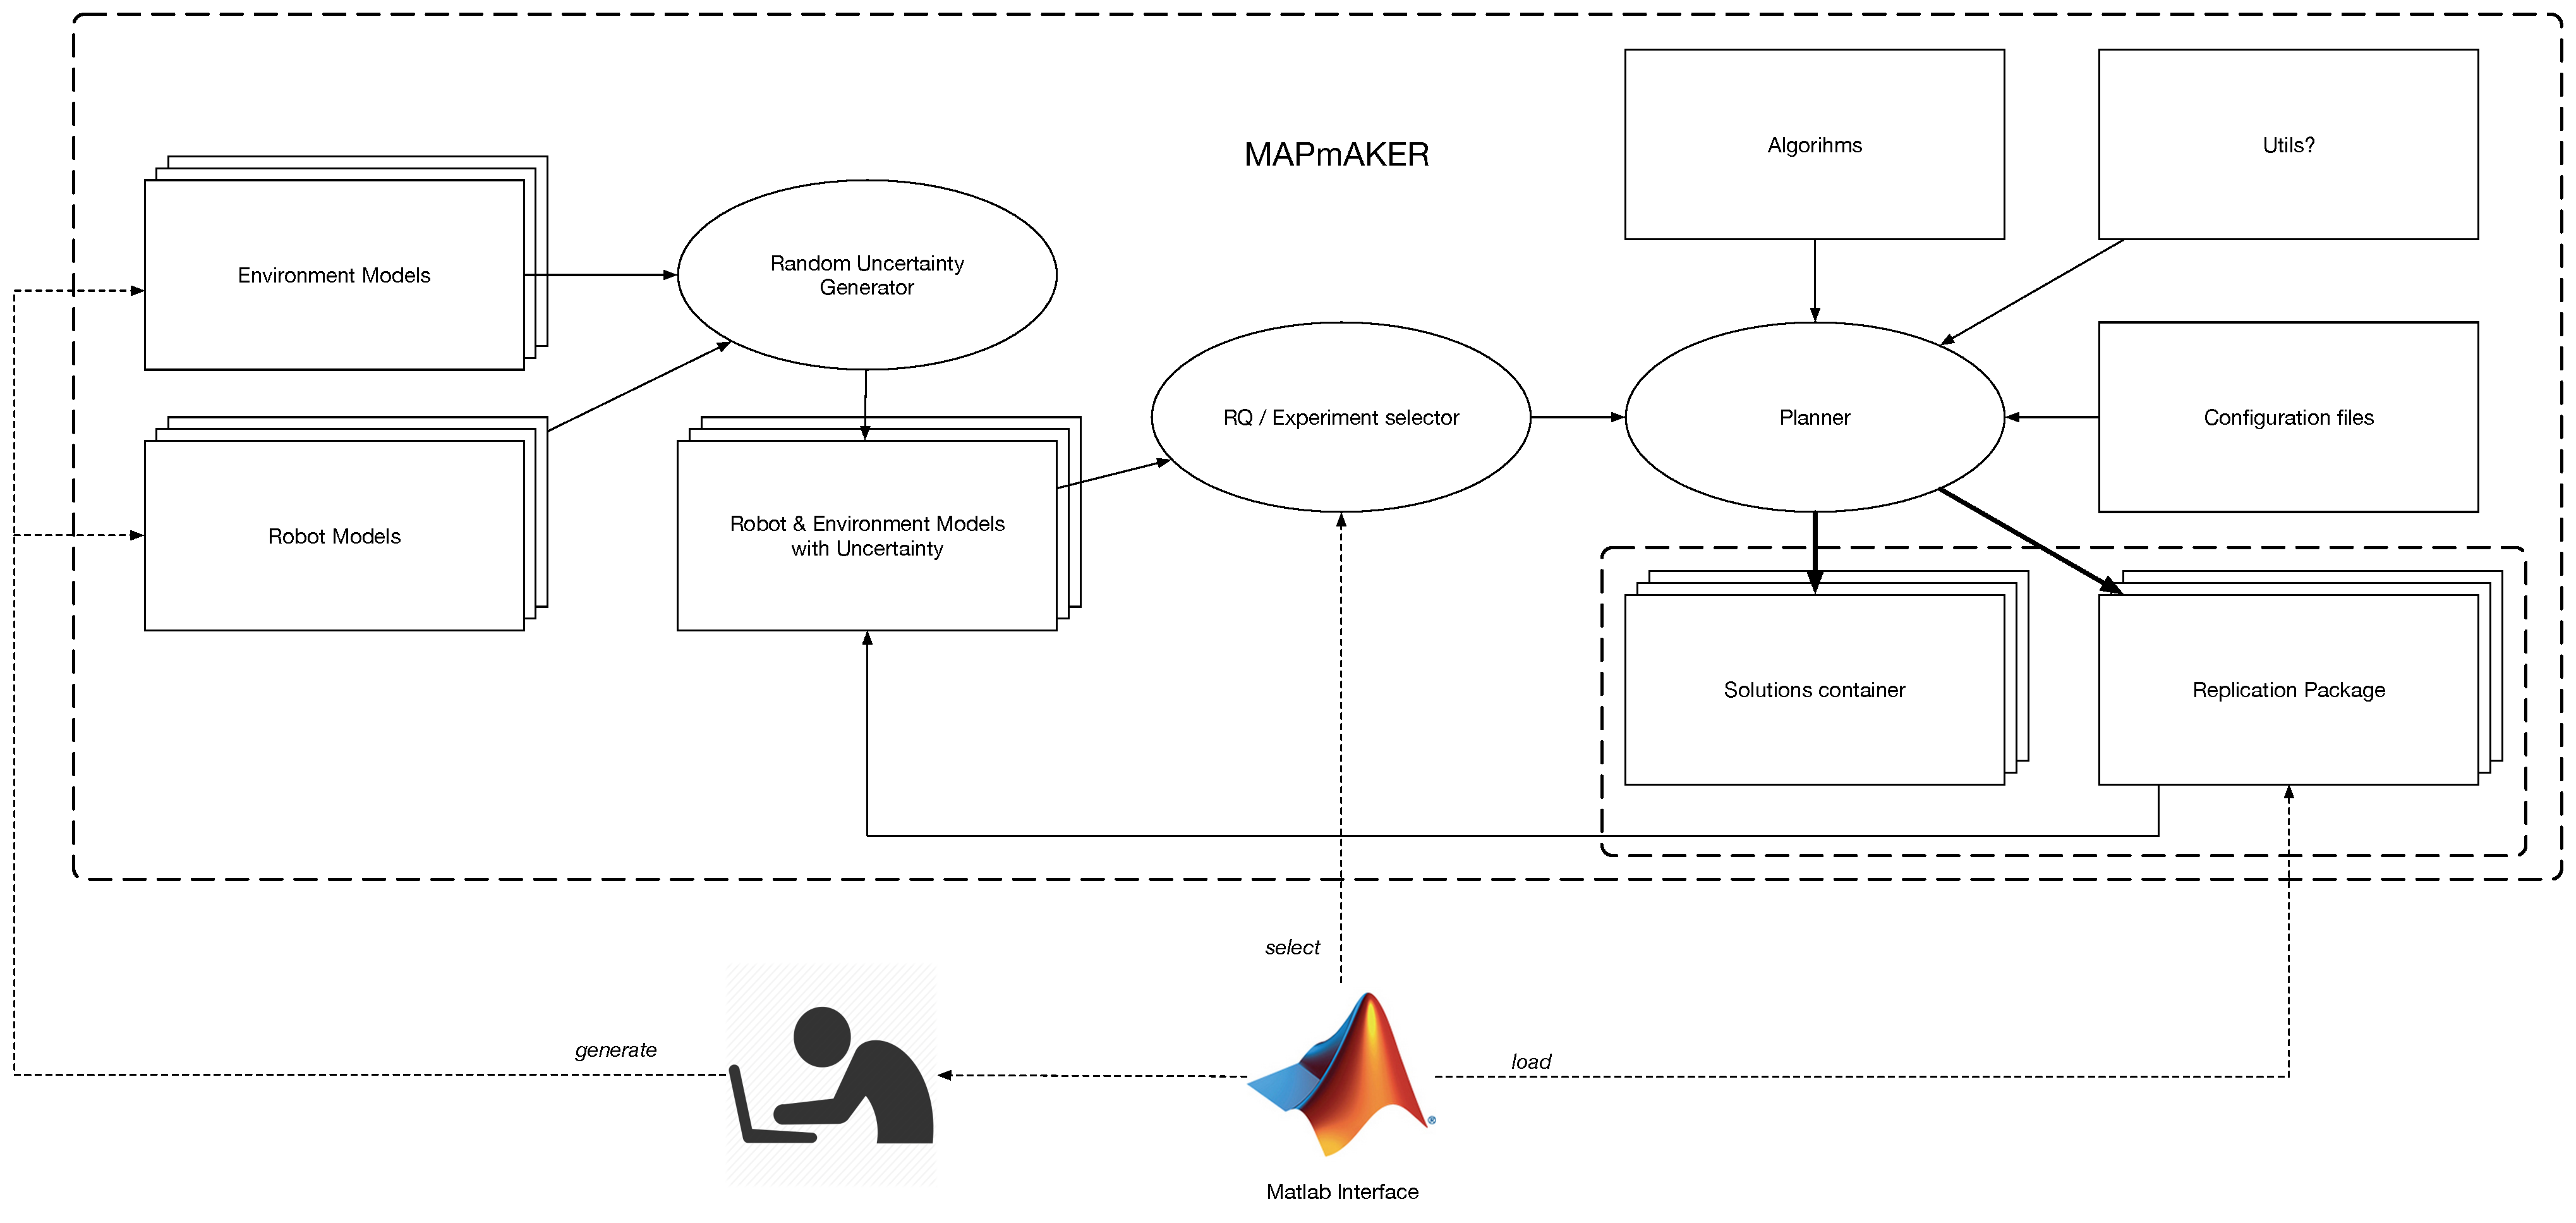
\includegraphics[width=1\linewidth]{Figures/MAPmAKER.pdf}
\caption{Overview of  MAPmAKER.}
\label{fig:overview}
\vspace{-.2cm}
\end{center}
\end{figure}




\textbf{Mission specification.}
Each robot is able to perform a complex mission, which is specified using an LTL formula.
This formula specifies how the services must be provided by the robots.
For example, a mission for a robot $r_1$ may require $r_1$ to  periodically load debris on $r_2$.
Thus, in order to allow robot $r_1$ to fulfill its mission, it is necessary that robots $r_1$ and $r_2$ synchronize their behaviours.





\textbf{Planning.} 
The \emph{Planner} uses the models of the robot(s) and the environment to compute plans that allow satisfying the missions of the robots.
%\ugh{The planner decomposes the robots within the robotic application}
It distributes the robots of the robotic application into subteams (i.e., ``dependency classes") based on the mission that each robot has to achieve.
Each dependency class contains a subset of robots that depend on each other for achieving their missions.
After  dependency classes are computed they are considered in isolation regarding the computation of plans. %that allow robots to satisfy their missions.

To compute a plan for a dependency class the  LTL formulae that are used to describe missions are evaluated on partial models.
Possible and definitive plans are computed by executing a classical planning algorithm twice: once for computing possible plans and once for computing definitive plans.
%The proposed algorithm There exists a subset of LTL formulae, known in literature as self-minimizing formulae



\textbf{Choosing between definitive and possible plans.}
The \emph{Plan selector} chooses between possible and definitive plans.
%The tool always try to reach the goal performing the lower number of actions.
%This work does not discuss how to choose between
%37 possible and de nitive plans. 
Several policies can be applied to choose between these plans.
Possible plans can be chosen only in cases in which a definitive plan is  not present.
Another policy may choose the plan with the shortest length, or it may consider non-functional aspects of the plans e.g., time to perform certain actions, or likelihood of detecting true or false evidence about partial information. 
In this work we assume  that the planner always chooses the shortest length plan. % between the possible and the definitive plan.
This policy may  reduce energy consumption. % every action performed by the robots may consume energy. 
%Thus, shorter plans require less energy.

\textbf{Detection of uncertain information.}
As robots perform actions and navigate within the environment, information regarding uncertain services and meeting capabilities can be detected.
Specifically, robots detect whether actions, services, and meeting capabilities are executable, provided, and possible, respectively.
\toolName\ updates the models of the robots and of the environment with the detected information.
Then, if needed, the planning algorithm is triggered and re-executed.
%This information is shared with the rest of the team so it can be take into account for further planning.







	
	\section{MApMAKER in Action}
	\label{sec:tool}
	
\toolName\  was developed as a  MATLAB~\cite{matlab} standalone application.
It is developed on top of an existing  planner presented in~\cite{tumova2016multi} which has been chosen since it already implements a decentralized planning procedure.
\toolName\ calls this planner twice considering two different versions of the model of the robots and their environments. 
The results obtained by performing this procedure are sound and correct.
Additional details and proofs can be found in~\cite{mapmaker17}.


\toolName\ can be executed in two ways, as shown in Listing~\ref{lst:command}.
\texttt{Scenario} is a Matlab file containing the model of the environment and the robots and \texttt{Experiment} encode the mission that must be satisfied by each robot.
The first option is the general way of executing the tool, using custom scenarios and experiments developed by the user.
In the second option the research question \texttt{RQ} that we tried to answer in this paper has to be specified.
This option is used for replicating the results that we present in~\cite{mapmaker17}.

\begin{lstlisting}[frame=single, backgroundcolor=\color{light-gray}, basicstyle=\footnotesize\ttfamily, language=Java, numbers=left, numberstyle=\tiny\color{black},caption= {Running \toolName}\label{lst:command}, captionpos=b]
mapmaker_exp 'Scenario', 'Experiment')
mapmaker_exp 'Scenario', 'Experiment', 'RQ')
\end{lstlisting}

%The tool is composed by several MATLAB-based scripts that can be executed independently for performing certain functions.
%In order to use \toolName it is sufficient to launch the function \emph{mapmaker\_exp} where the \emph{research question}, the \emph{example} or map of the environment and the \emph{experiment} to check are their arguments.
%This function enormously simplifies the performance of the tool, but there are other functionalities that can also be exploited explained in the previous section.





%In a normal case where the scenarios are already defined, the only components of the architecture depicted in~\ref{fig:overview} that are used are the \emph{Replication Package}, the \emph{Robot \& Environment models with uncertainty}, the \emph{Planner} itself and its inputs and, of course, the \emph{Solutions container}.
%The first component represents a folder where the models of the robot and environment with a certain added uncertainty for the selected experiment are stored.

When  \toolName\ is launched a graphical interface similar to the one presented  in Figure~\ref{fig:outputexample} is showed.
The grid represents the environment in which robot are moving.
Each cell represents a location of the environment and has a number associated, as labeled in some of them.
Robots are represented by the squared colored boxes.
Actions are used to encode movement, i.e., each robot can move left, right, up and down.
A robot  cannot move between adjacent cells if they are separated by thick bordered lines.
Whenever  it is unclear if a robot can move between adjacent cells, these cells are separated by a red border.
Each service is associated with a number.
Whenever a service can be provided by a robot in a cell, the cell is labeled with the corresponding number.
Finally, synchronization capabilities are represented by a black cross.
If it is unclear if two robots can synchronize in a cell, the cell is labeled with a green cross.
The graphical interface shows the plan execution.
Assume for example that the robots $r_1$, $r_2$ and $r_3$ have the following \emph{local missions}.
Robot $r_1$ has to perform the action 1, which is present in cells 7 and 9---note that the missions associated with each robot are colored with the color used for representing the robot.
Action 1 and action 2 (which has to be accomplished by robot $r_2$) are located in a cell labeled with a cross, so robot must meet there and perform both actions at the same time.
Robot $r_1$ can also perform this mission in cell 9, but it is unsure the synchronization in this cell.
As explained before, robot $r_2$ must synchronize with robot $r_1$ and perform action 2, but then it has to reach cell 22 for performing action 3.
Finally, robot $r_3$ has to perform action 4 in cell 2 and action 5, which can be possibly executed in cell 18 or in cell 30.

In figure~\ref{fig:outputexample} we represented different plans performed by the robots. 
Starting from robot $r_1$, there are two different plans that could be performed.
P1 represents a definitive plan and P1' a possible plan where a true evidence was detected by the robot.
In those paths the robot basically reaches the cell where the action can be performed with the help of robot $r_2$ and moves away. 
In both cases the plan is repeated continuously.
For robot $r_2$ we represented two different paths as well.
P2 represents a possible plan ---due to the uncertainty of the door between cells 14 and 20--- where $r_2$ synchronizes with $r_1$ in order to accomplish action 2.
P2' is a similar path with the difference that the synchronization is performed in cell 9, where the it is uncertain.
In both cases the plan is repeated continuously.
Finally, P3 represents a possible path where robot $r_3$ accomplishes action 4 and then action 5 in cell 18.
Then, it performs the same action continuously.
\sergio{label paths in the picture}
We produced a video that shows how to execute the tool and its performance. 
It is available in~\footnote{https://goo.gl/jYeLbm}.

%The results achieved and presented in~\cite{mapmaker17} can be replicated using this models.
%They are loaded and set as MATLAB workspace variables in the second component.

%The planner needs as input the information from this variables and also from the scripts \emph{Algorithms}, \emph{Utils} and \emph{Configuration files}, that are automatically linked.
%During the execution of the planner \sergio{image representing the execution of the tool?} the MATLAB interface shows a window with the goals of the current mission. 
%Furthermore, after the computation of the plan it shows the movements of the robots and their knowledge of the environment.
%When all the robots have reached their goals or they realized that their local mission is not feasible the experiments concludes.
%Once the experiment is concluded, the data extracted (as explained in~\ref{sec:approach}) is stored in the solutions container component.


\begin{figure}[t]
\begin{center}
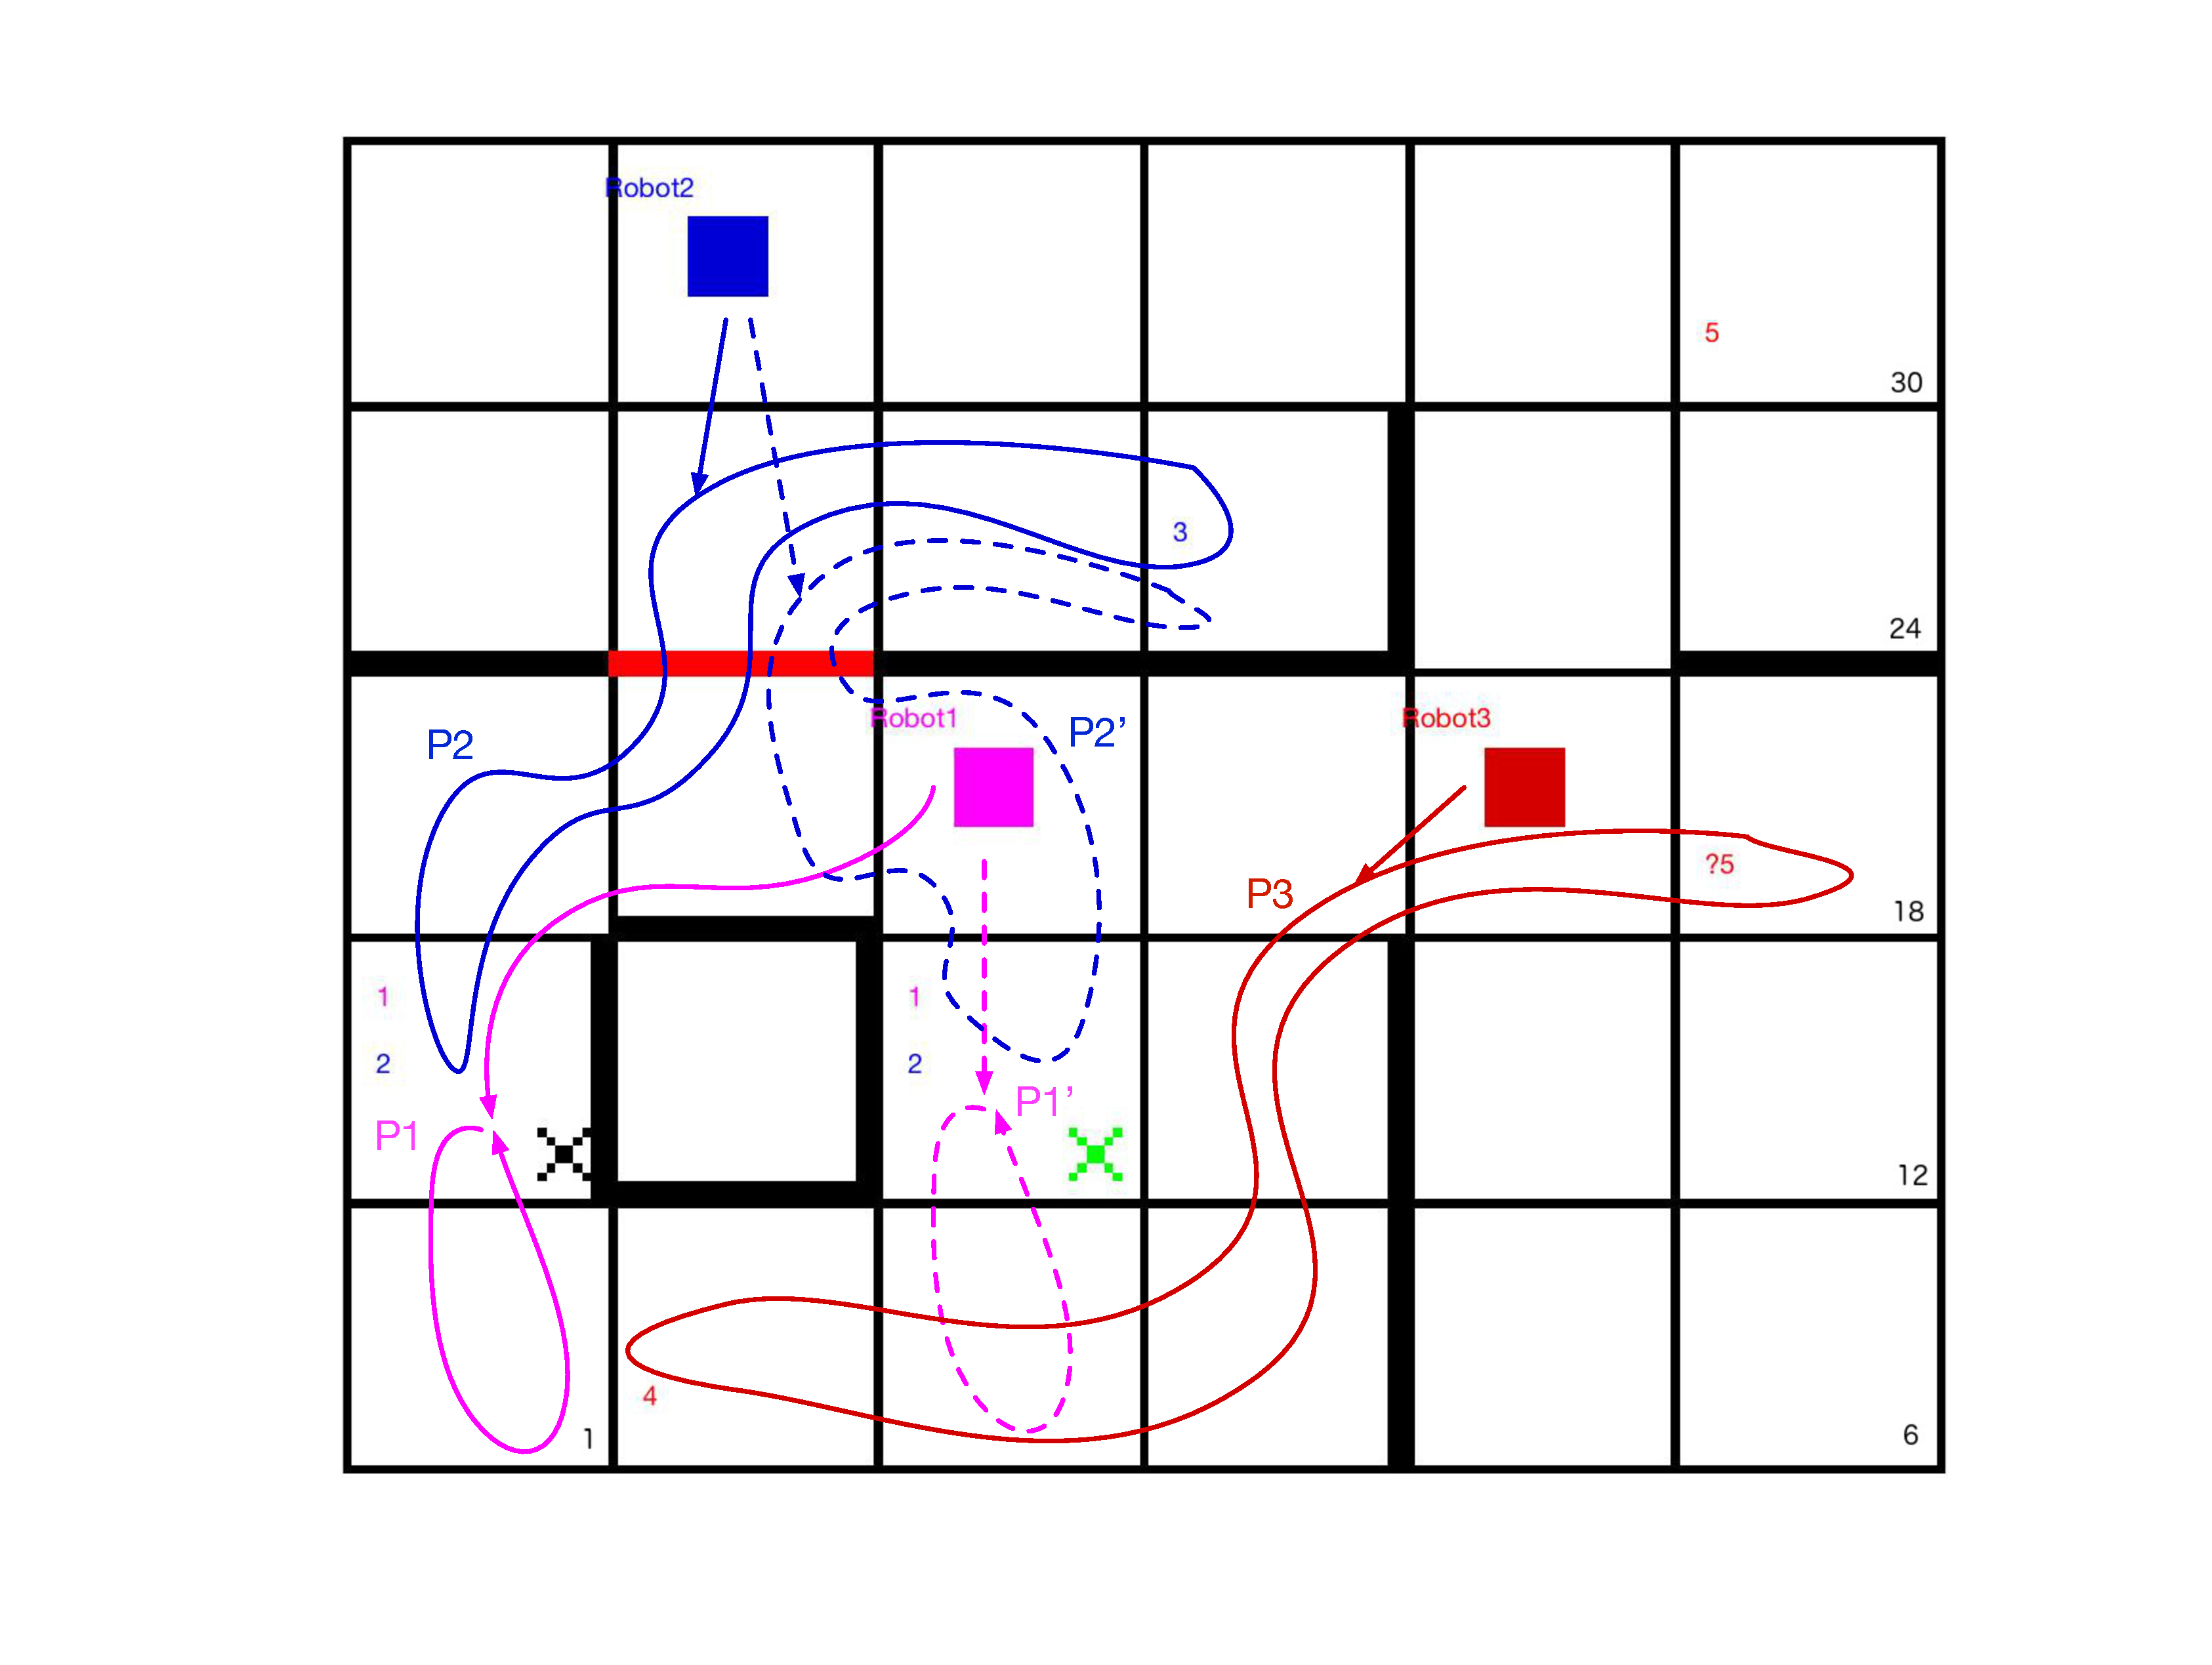
\includegraphics[width=1\linewidth]{Figures/arrows.pdf}
\caption{\toolName\ usage scenario.}
\label{fig:outputexample}
\end{center}
\end{figure}

%In~\cite{mapmaker17}  we have shown that our tool is able to perform a plan even in environments full of uncertainty.
%Thus, \toolName~ is able to compute a plan where other planners will not.
%However, the computation time and the number of actions to be performed by the robot that tries to follow a possible plan and detects a false evidence are normally greatly increased.
%This increasing is due to required re-computing that has to be performed when looking for a new possible plan.

%For checking its performance the tool was tested in different environments based on real-world scenarios.
%The model of the uncertainty of the environment was randomly created and matched with randomly models of the robots (service and synchronization locations and uncertainties).
%The performance of tool was evaluated in two Research Questions divided in three experiments (one for each kind of uncertainty defined for this project).
%The results are presented and discussed in~\cite{mapmaker17}.

%\textbf{Tool Validation}



	
	
	\section{Evaluation}
	\label{sec:evaluation}
	

To evaluate  \toolName\ we formulate a research question,
\textbf{RQ}: Is MAPmAKER able to perform planning in partially known environments?
%\textbf{RQ1}: How does MAPmAKER help planning in partially known environments? \textbf{RQ2}: How does the employed decentralized algorithm help in plan computation?
%The full evaluation might be found in~\cite{menghi2018multi}. 
To answer it, we  had considered the simulated scenario introduced in Sec.~\ref{sec:tool}.
We created a partial robot application starting from the models of the robots and their environment.
We then introduced uncertainty in the three considered dimensions introduced in Sec.~\ref{sec:approach}.
Examples of such uncertainties are whether the system has certain knowledge about the transition through doors (e.g., the one between cells 37 and 38 in Fig.~\ref{fig:runningexample}) or about the provision of services (e.g., \emph{deliver} at cells 24 and 26).
We introduced uncertainty through a random process and created three different scenario configurations based on the same scenario.
We also randomized the initial position of each robot, creating three different sets of initial configurations.
The nine experiments we performed to validate \toolName~consist of the nine possible combinations of the scenario and initial configurations.

The results show that the decentralized algorithm actually helps in improving performances.
The results show that \toolName~is able to compute plans in situations where traditional planners cannot. 
Furthermore, \toolName also improves the performance in terms of plan length in many situations since it may consider more planning options.
In the folder \texttt{ResultsPaperRoSE} \patrizio{which folder?} we provide a set of videos showing the performance of \toolName~in these experiments.
We also provide results, containing computation time, plan length, false and true evidences found by the robots, and ratio between the definitive and possible plans in terms of computation time and plan length.
The evaluation of the underlying algorithms might be found in~\cite{menghi2018multi}. 

%a set of existing examples: one obtained from the RoboCup Logistics League competition~\cite{karrasrobocup} and an apartment of a large residential facility for senior citizens~\cite{map}.
%We created a partial robot application starting from the models of the robots and their environment contained in these examples.
%We performed different experiments in which we evaluated the impact of partial information about the action execution, services provisioning and meeting capabilities on the planning procedure.
%We compare whether computing possible plans actually helps mission achievement.
%
%To answer RQ2 we analyzed the advantages of the decentralized procedure provided by \toolName.
%We had considered the set of partial models considered in the previous experiments. 
%We added an additional robot, i.e., robot $r_3$, which has a mission that can be achieved without collaborating with neither  robot $r1$ nor with robot $r2$. 
%We then executed \toolName\ with the decentralized procedure enabled (computing two different dependency classes based on the collaboration among robots) and disabled (all the robots are part of the same dependency class). 
%Then, we compare each performance. 
%
%We performed three experiments for each scenario, each of them unique since the generator associates a random uncertainty and an initial position of the robotic team to each of them (by using the given \texttt{randomModelGenerator} function).

%To answer RQ1 we  had considered a set of existing examples:
%one obtained from the RoboCup Logistics League competition~\cite{karrasrobocup} and an apartment of a large residential facility for senior citizens~\cite{map}.
%We created a partial robot application starting from the models of the robots and their environment contained in these examples.
%We performed different experiments in which we evaluated the impact of partial information about the action execution, services provisioning and meeting capabilities on the planning procedure.
%We compare whether computing possible plans actually helps mission achievement.
%This is done by comparing our planner with one that is only able to compute definitive plans.
%The results can be summarized as follows.
%\toolName\ is effective when  a possible plan is selected, and the robot discovers during the plan execution 
%that unknown actions, services, and meeting capabilities are executable, provided, and possible, respectively.
%%\toolName\ \ugh{is also effective in the cases in which a possible plan  is computed, it can actually be performed and a classical planning algorithm cannot compute a definitive plan.} 
%\toolName\ is also effective when this three conditions are given:
%\begin{enumerate*}
%\item a possible plan is computed;
%\item the possible plan can actually be performed; and 
%\item a classical planning algorithm cannot compute a definitive plan.
%\end{enumerate*}
%This situation occurs in the cases in which the only way to fulfill a mission involves some partial information present in the model.
%When \toolName\ chooses a definitive plan, it is as effective as a classical planner that is only able to compute definitive plans.
%The computation time and the length of plans are increased whenever  a possible plan is chosen but unknown actions, services, and meeting capabilities turned to be not executable, provided, and possible, respectively.
%More information about the considered examples, experimental set up, and the obtained results can be found in~\cite{menghi2018multi}.
%
%To answer RQ2 we analyzed the advantages of the decentralized procedure provided by \toolName.
%We had considered the set of partial models considered in the previous experiments. 
%We added an additional robot, i.e., robot $r_3$, which has a mission that can be achieved without collaborating with neither  robot $r1$ nor with robot $r2$. 
%We then executed \toolName\ with the decentralized procedure enabled and disabled. 
%Then, we compare each performance. 
%When \toolName\ was executed with the  decentralized procedure it computed two dependency classes; one containing robots $r_1$ and $r_2$ and one containing robot $r_3$. 
%Viceversa, when the decentralized procedure was disabled, \toolName\ 
%analyzed a single team containing  robots $r_1$, $r_2$, and $r_3$. 
%The results show a drastic improvement in the efficiency of \toolName\ when the decentralized procedure was enabled.
%More information can be found in~\cite{menghi2018multi}.

%Then, the \emph{Random model generator} generates a certain number (defined by the user) of tests based on the previously explained models.
%Each of this tests is unique since the generator associates a random uncertainty and an initial position of the robotic team to each of them.
%This process is automatically performed for each experiment, since the uncertainty that is checked changes between them (e.g. execution of transitions in \emph{Experiment 1}, services provisioning in \emph{Experiment 2} and meeting capabilities in \emph{Experiment 3}).
%The generation of models must be performed once, although we provide an already working set in our repository and this step can be skipped.
%The already existing models of the environment represent models of real robot applications, i.e., the RoboCup Logistics League competition~\cite{karrasrobocup} and an apartment of a large residential facility for senior citizens~\cite{map}.
%This set is stored in the folder "ReplicationPackage", where the new scenarios must be saved as well.


	
	
	\section{Conclusions}
	\label{sec:conclusion}
	We presented  \toolName, a  decentralized planner for partially known environments.
%\del{The theoretical results show that any planner can be used within \toolName. %\toolName\ does not aim to compete with state of the art planners. It is realized as a proof of concepts to show that (i) models containing partial information can be efficiently handled in by current planners and that (ii) decentralized procedures help in improving performances.} 
The \toolName\ implementation relies on a naive implementation of a planner that comes from literature and has been customized within the proposing framework.
 %\toolName\ solves the decentralized planning problem when partial robot applications are analyzed.
Our evaluation showed how  \toolName\ improves planning in cases in which partial information is present.
%We also showed that the implemented decentralized procedure improves the performance of the planning algorithm.

As future work we will experiment with more complex scenarios and with real robots.
To do so, we will use more efficient planners to speed up the computation.
Other work will include the study of appropriate policies to select between definitive and possible plans.




	\balance
	\bibliographystyle{IEEEtran}
	\bibliography{sigproc}
	
\end{document}
